\documentclass[assignment2.tex]{subfiles}
\begin{document}

\section*{1η Άσκηση}
Ζητείται να βρεθούν όλες οι ρίζες της συνάρτησης $f(x)=x^2 + 10\cos x$ με τη μέθοδο του σταθερού σημείου. Καταρχάς, είναι σημαντικό να σημειωθεί ότι η $f$ είναι άρτια (\ref{eq:even}), αφού είναι άθροισμα άρτιων συναρτήσεων. Επομένως, αν $\rho_1>0$ είναι ρίζα της εξίσωσης, τότε και η $-\rho_1$ θα είναι ρίζα.
\begin{equation}
f(-x) = (-x)^2 + 10 \cos (-x) = x^2 + 10 \cos x = f(x)
\label{eq:even}
\end{equation} 

Επειδή η $x^2$ απειρίζεται για $x\rightarrow \infty$ και $|10\cos x|\leq 10$, αναμένεται ότι οι όποιες ρίζες της $f$ θα βρίσκονται γύρω από την αρχή των αξόνων. Στο Σχήμα \ref{fig:f1} δίνεται το γράφημα της $f$, όπου φαίνεται ότι τέμνει τον $x$ άξονα 4 φορές και μάλιστα οι ρίζες είναι ανά δύο συμμετρικές ως προς το $O$.
\begin{figure}[hp]
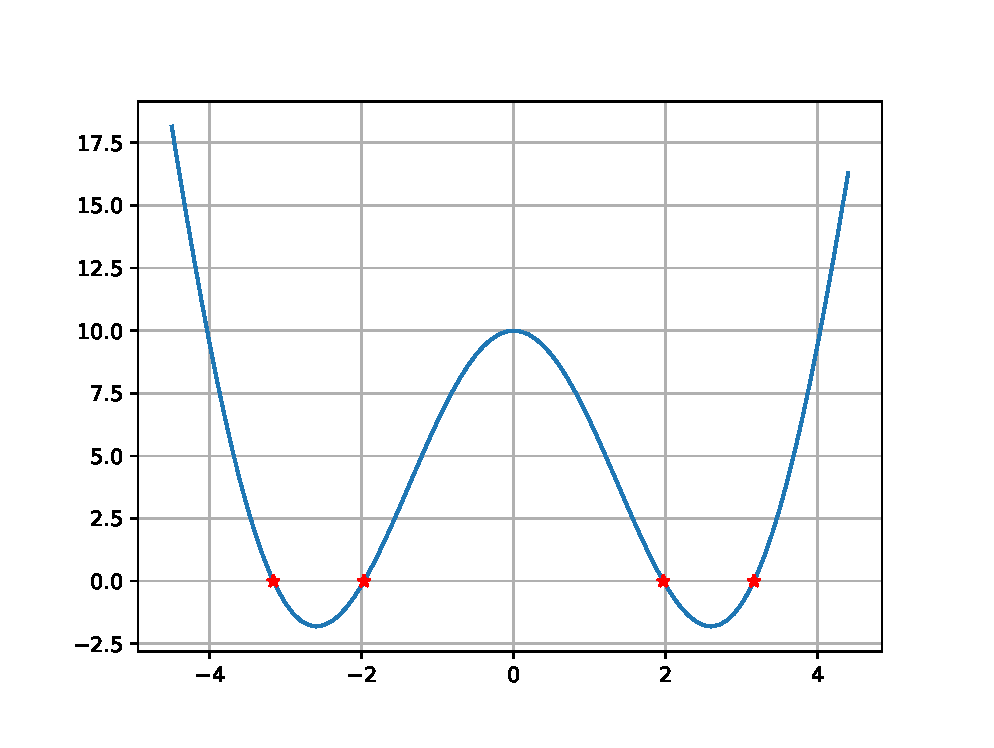
\includegraphics[width=0.7\textwidth]{f1.eps}
\centering
\caption{Γράφημα $x^2+10\cos x$ γύρω από το $O(0,0)$}
\label{fig:f1}
\end{figure} 

Για επίλυση με τη μέθοδο σταθερού σημείου, υπάρχουν διάφορες επιλογές για την $g(x)$, όπου $x=g(x)\leftrightarrow f(x)=0$. Αυτές είναι:

\begin{enumerate}
\item 
\begin{equation}
g(x)=x - f(x) \rightarrow g(x)=x - x^2 -10\cos x
\end{equation}
\item 
\begin{equation}
\begin{split}
x^2&+10 \cos x =0 \rightarrow \\
x^2 &=-10\cos x \rightarrow \\
x &= -10\frac{\cos x}{x} \rightarrow \\
g(x) &= -10\frac{\cos x}{x}
\end{split}
\end{equation}
\item 
\begin{equation}
\begin{split}
x^2&+10 \cos x =0 \rightarrow \\
x^2 &=-10\cos x \rightarrow \\
x &= \pm\sqrt{-10\cos x} \rightarrow \\
g(x) &= \pm\sqrt{-10\cos x}
\end{split}
\end{equation}
\item 
\begin{equation}
\begin{split}
x^2&+10 \cos x =0 \rightarrow \\
\cos x &=-\frac{x^2}{10} \rightarrow \\
x &=  \arccos \left(-\frac{x^2}{10}\right) \rightarrow \\
g(x) &= \arccos \left(-\frac{x^2}{10}\right)
\end{split}
\end{equation}
\end{enumerate}

Για να συγκλίνει η μέθοδος του σταθερού σημείου σε μια ρίζα της $f$ για κάποια από τις παραπάνω συναρτήσεις, πρέπει $|g'(x)|<1$ για $x\in(a, b)$, όπου το διάστημα $(a,b)$ περιέχει τη ρίζα της $f$.

Από τη γραφική παράσταση της $f$, μπορούν να αναζητηθούν οι θετικές ρίζες στα διαστήματα $(1.95, 2.5)$ και $(2.5, 3,2)$. Σε αυτά τα διαστήματα δεν πληρούν όλες οι πιθανές $g$, το κριτήριο σύγκλισης. Στο διάστημα $I_1=(1.95, 2.5)$ επιλέγεται η $g_1(x)=\arccos \left(-\frac{x^2}{10}\right)$ και στο διάστημα $I_2=(2.5, 3,2)$ επιλέγεται η $g_2(x)=\sqrt{-10\cos x}$.

Στο Σχήμα \ref{fig:dg1_dg2} δίνεται η γραφική παράσταση των παραγώγων $g_1'$ και $g_2'$. Όπως φαίνεται, και για τις δύο συναρτήσεις ισχύει $|g_i'(x)|<1$, στα διαστήματα $I_1$ και $I_2$.
\begin{figure}[hp]
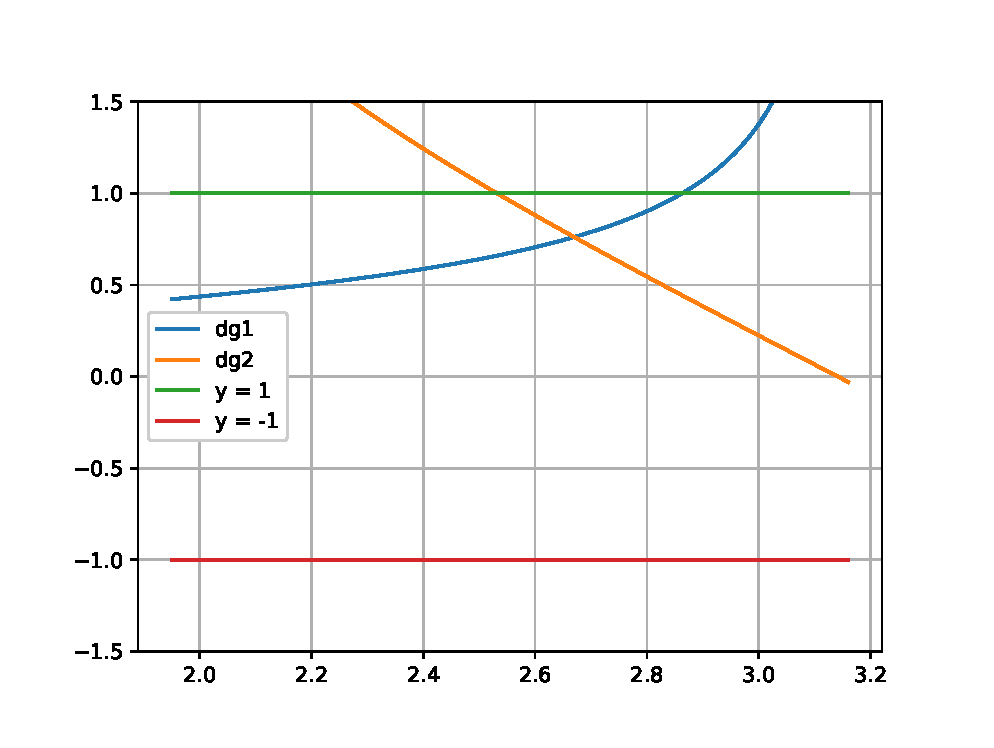
\includegraphics[width=0.7\textwidth]{dg1_dg2.eps}
\centering
\caption{$g_1'$ και $g_2'$ κοντά στις ρίζες της $f$}
\label{fig:dg1_dg2}
\end{figure} 

Ο αλγόριθμος της μεθόδου σταθερού σημείου εκτελέστηκε για $g_1$ και $g_2$ και τα αποτελέσματα του δίνονται στον Πίνακα \ref{table:fixed_point} με ακρίβεια $10^{-4}$. Όπως προαναφέρθηκε, ο προσδιορισμός των δύο θετικών ριζών επιτρέπει τον ταυτόχρονο προσδιορισμό και των αρνητικών και μάλιστα χωρίς επιπλέον υπολογιστικό κόστος.

\begin{table}[ht]
\centering
\begin{tabular}{||c c c||} 
	\hline
	$g_i$& $\rho>0$ & $\rho<0$ \\ [0.5ex] 
	\hline\hline
	$\arccos \left(-\frac{x^2}{10}\right)$ & 1.9689 & -1.9689 \\ 
	\hline
	$\sqrt{-10\cos x}$ & 3.1619 & -3.1619 \\ [1ex] 
	\hline
\end{tabular}
\caption{Αποτελέσματα Προσομοίωσης}
\label{table:fixed_point}
\end{table}

Παρακάτω ακολουθεί ο κώδικας που γράφτηκε σε \textlatin{Python} και έγινε χρήση της βιβλιοθήκης \textlatin{Numpy}.
\selectlanguage{english}
\lstinputlisting[style=python, firstline=8]{ex1.py}
\end{document}